%   MSc Business Analytics Dissertation
%   Format based on skeleton template provided as part of module MIS40750
%
%   Title:     Optimising the design of buffer preparation in bioprocessing
%              facilities
%   Author:    Sean Tully
%
%   Appendix 3: real-world example 1
%
%   Change Control:
%   When     Who   Ver  What
%   -------  ----  ---  --------------------------------------------------------

\chapter{Real-world data set 1}\label{C.real1}

\begin{table}[h]
    \centering Table A1: Buffer data for real-world data set 1\\
    \label{tbl.buffer1}
    \begin{tabular}{l | c | c | c}
        names & required volumes & use start times & use durations\\
        & $U_{n}$ (l) & $t_{\mathit{USE},n}^{*}$ (h) 
        & $\Delta t_{\mathit{USE},n}$
        (h)\\ \hline
        \text{Buffer \#1} & \SI{19676.0}{} & \SI{733.87}{} & \SI{48.99}{}\\
        \text{Buffer \#2} & \SI{18528.0}{} & \SI{644.18}{} & \SI{36.95}{}\\
        \text{Buffer \#3} & \SI{17346.0}{} & \SI{684.60}{} & \SI{49.27}{}\\
        \text{Buffer \#4} & \SI{15055.0}{} & \SI{794.96}{} & \SI{28.01}{}\\
        \text{Buffer \#5} & \SI{13896.0}{} & \SI{628.54}{} & \SI{52.59}{}\\
        \text{Buffer \#6} & \SI{10267.0}{} & \SI{728.99}{} & \SI{53.12}{}\\
        \text{Buffer \#7} & \SI{10070.0}{} & \SI{677.94}{} & \SI{20.86}{}\\
        \text{Buffer \#8} & \SI{6797.0}{} & \SI{728.99}{} & \SI{53.12}{}\\
        \text{Buffer \#9} & \SI{6716.0}{} & \SI{612.90}{} & \SI{70.40}{}\\
        \text{Buffer \#10} & \SI{4632.0}{} & \SI{645.50}{} & \SI{35.63}{}\\
        \text{Buffer \#11} & \SI{3780.0}{} & \SI{729.34}{} & \SI{43.19}{}\\
        \text{Buffer \#12} & \SI{3694.0}{} & \SI{678.92}{} & \SI{42.17}{}\\
    \end{tabular}
\end{table}

\begin{table}[h]
    \centering Table A2: Vessel data for real-world data set 1\\
    \label{tbl.vessel1}
    \begin{tabular}{l | r | r}
        names & volumes & costs\\
        & $V_{m}$ (l) & $c_{m}$ (--)\\\hline
        \SI{2000}{\litre} & \SI{2222.0}{} & \SI{95.64}{}\\
        \SI{4000}{\litre} & \SI{4444.0}{} & \SI{144.96}{}\\
        \SI{5000}{\litre} & \SI{5556.0}{} & \SI{165.72}{}\\
        \SI{8000}{\litre} & \SI{8889.0}{} & \SI{219.71}{}\\
        \SI{10000}{\litre} & \SI{11111.0}{} & \SI{251.19}{}\\
        \SI{12000}{\litre} & \SI{13333.0}{} & \SI{280.83}{}\\
        \SI{15000}{\litre} & \SI{16667.0}{} & \SI{320.37}{}\\
        \SI{20000}{\litre} & \SI{22222.0}{} & \SI{380.73}{}\\
        \SI{25000}{\litre} & \SI{27778.0}{} & \SI{435.28}{}\\
    \end{tabular}
\end{table}

\begin{table}[h!]
    \centering Table A3: Global parameters for real-world data set 1
    \label{tbl.parameters1}
    \begin{tabular}{l | l | r | c}
        symbol & short description & value & unit\\ \hline
        $T$ & process cycle time & 96.0 & h\\
        $\Delta t_{\mathit{PREP,PRE}}$ & prep pre duration & 11.0 & h\\
        $\Delta t_{\mathit{PREP,POST}}$ & prep post duration & 2.5 & h\\
        $\Delta t_{\mathit{TRANSFER}}$ & transfer duration & 2.2 & h\\
        $\Delta t_{\mathit{HOLD,PRE}}$ & hold pre duration & 9.0 & h\\
        $\Delta t_{\mathit{HOLD,POST}}$ & hold post duration & 1.0 & h\\
        $\Delta t_{\mathit{HOLD,MIN}}$ & minimum hold duration & 12.0 & h\\
        $\Delta t_{\mathit{HOLD,MAX}}$ & maximum hold duration & 60.0 & h\\
        $f_{\mathit{MINFILL}}$ & minimum fill ratio & 0.27 & --\\
        $f_{\mathit{UTIL}}$ & maximum utilisation ratio & 0.7 & --\\
    \end{tabular}
\end{table}

\begin{figure}[h]
    \centering
    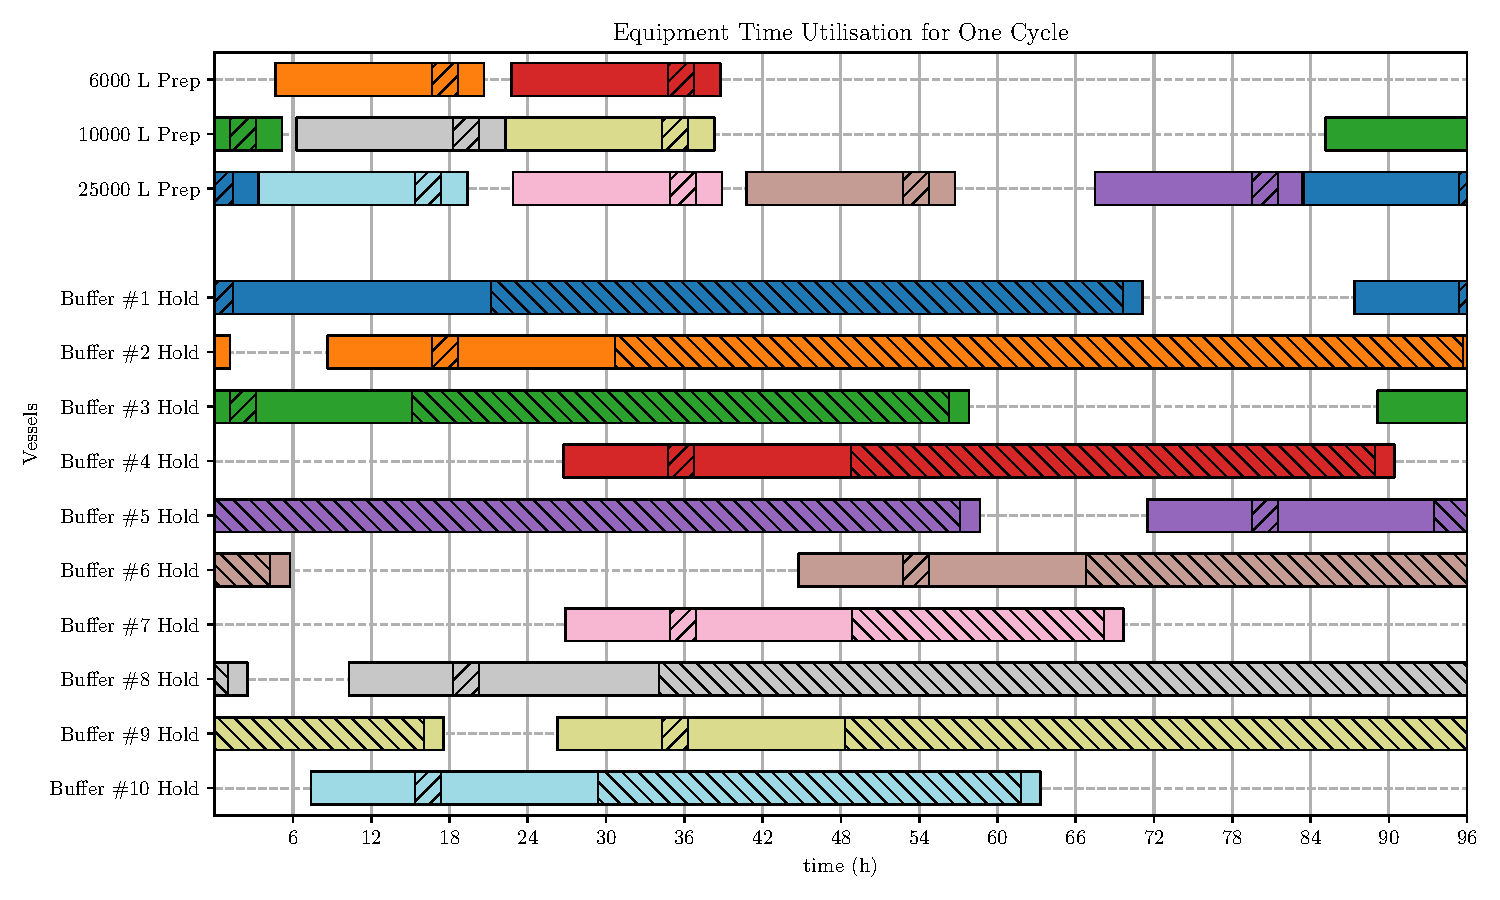
\includegraphics[width=\linewidth]{../examples/plant1/plot2.pdf}
    Figure A1: Real-world data set 1 -- complete model with minimised
        hold times
    \label{fig.secondary1}
\end{figure}
